\begin{appendices}

%Some Table of Contents entry formatting
\addtocontents{toc}{\protect\renewcommand{\protect\cftchappresnum}{\appendixname\space}}
\addtocontents{toc}{\protect\renewcommand{\protect\cftchapnumwidth}{6em}}

%Begin individual appendices, separated as chapters

\chapter{Supporting information for Chapter 2}
This appendix compares the experimental results between pure dielectric particles and  Janus particles undergoing CCEP. The results demonstrate the partial charge on the dielectric semi sphere of Janus Particle, which may explain the variation in the particles’ lateral displacement during oscillation. The theoretical details of electrostatics and low Reynolds number hydrodynamics are also shown to support out plausible mechanism of directed motion in Chapter 2.  


\section{\new{Additional Experiments and Estimates}}


%%%%%%%%%%%%%%%%%%%%%%%%%%%%%%
%%%%%%%%%%%%%%%%%%%%%%%%%%%%%%
\subsection{\new{CCEP Dynamics of Dielectric (non-Janus) Particles}} \label{sec:Dielectric}

As a control experiment, we examined the behavior of bare silica particles ($8~\mu\text{m}$ diameter) in mineral oil when subject to an applied electric field.
Surprisingly, these insulating particles also oscillated between the two electrodes but at much lower frequencies than the metal-coated particles.
For an applied voltage $V=800~\text{V}$ and electrode separation $H=200~\mu\text{m}$, silica particles oscillated with a average frequency of ${\sim}0.1~\text{Hz}$ as compared to ${\sim}100~\text{Hz}$ for similar metallodielectric Janus particles (Fig.~\ref{fig:Silica}a). 
Dielectric particles spent most of their time at the electrode surface before rapidly moving off towards the opposite electrode.
We examined the characteristic time $\tau$ required for a particle near the electrode surface to leave the focal plane of the microscope (Fig.~\ref{fig:Silica}a,b).
This time was of order $\tau\sim 5~\text{ms}$ for both Janus and dielectric particles, indicating that the different particles moved at similar velocities.
These observations suggest that Janus particles and dielectric particles acquire similar amounts of charge but at different rates.
Further study is required to better characterize and understand the charging of dielectric materials on contact with biased electrodes.

\begin{figure}[h]
    \centering
    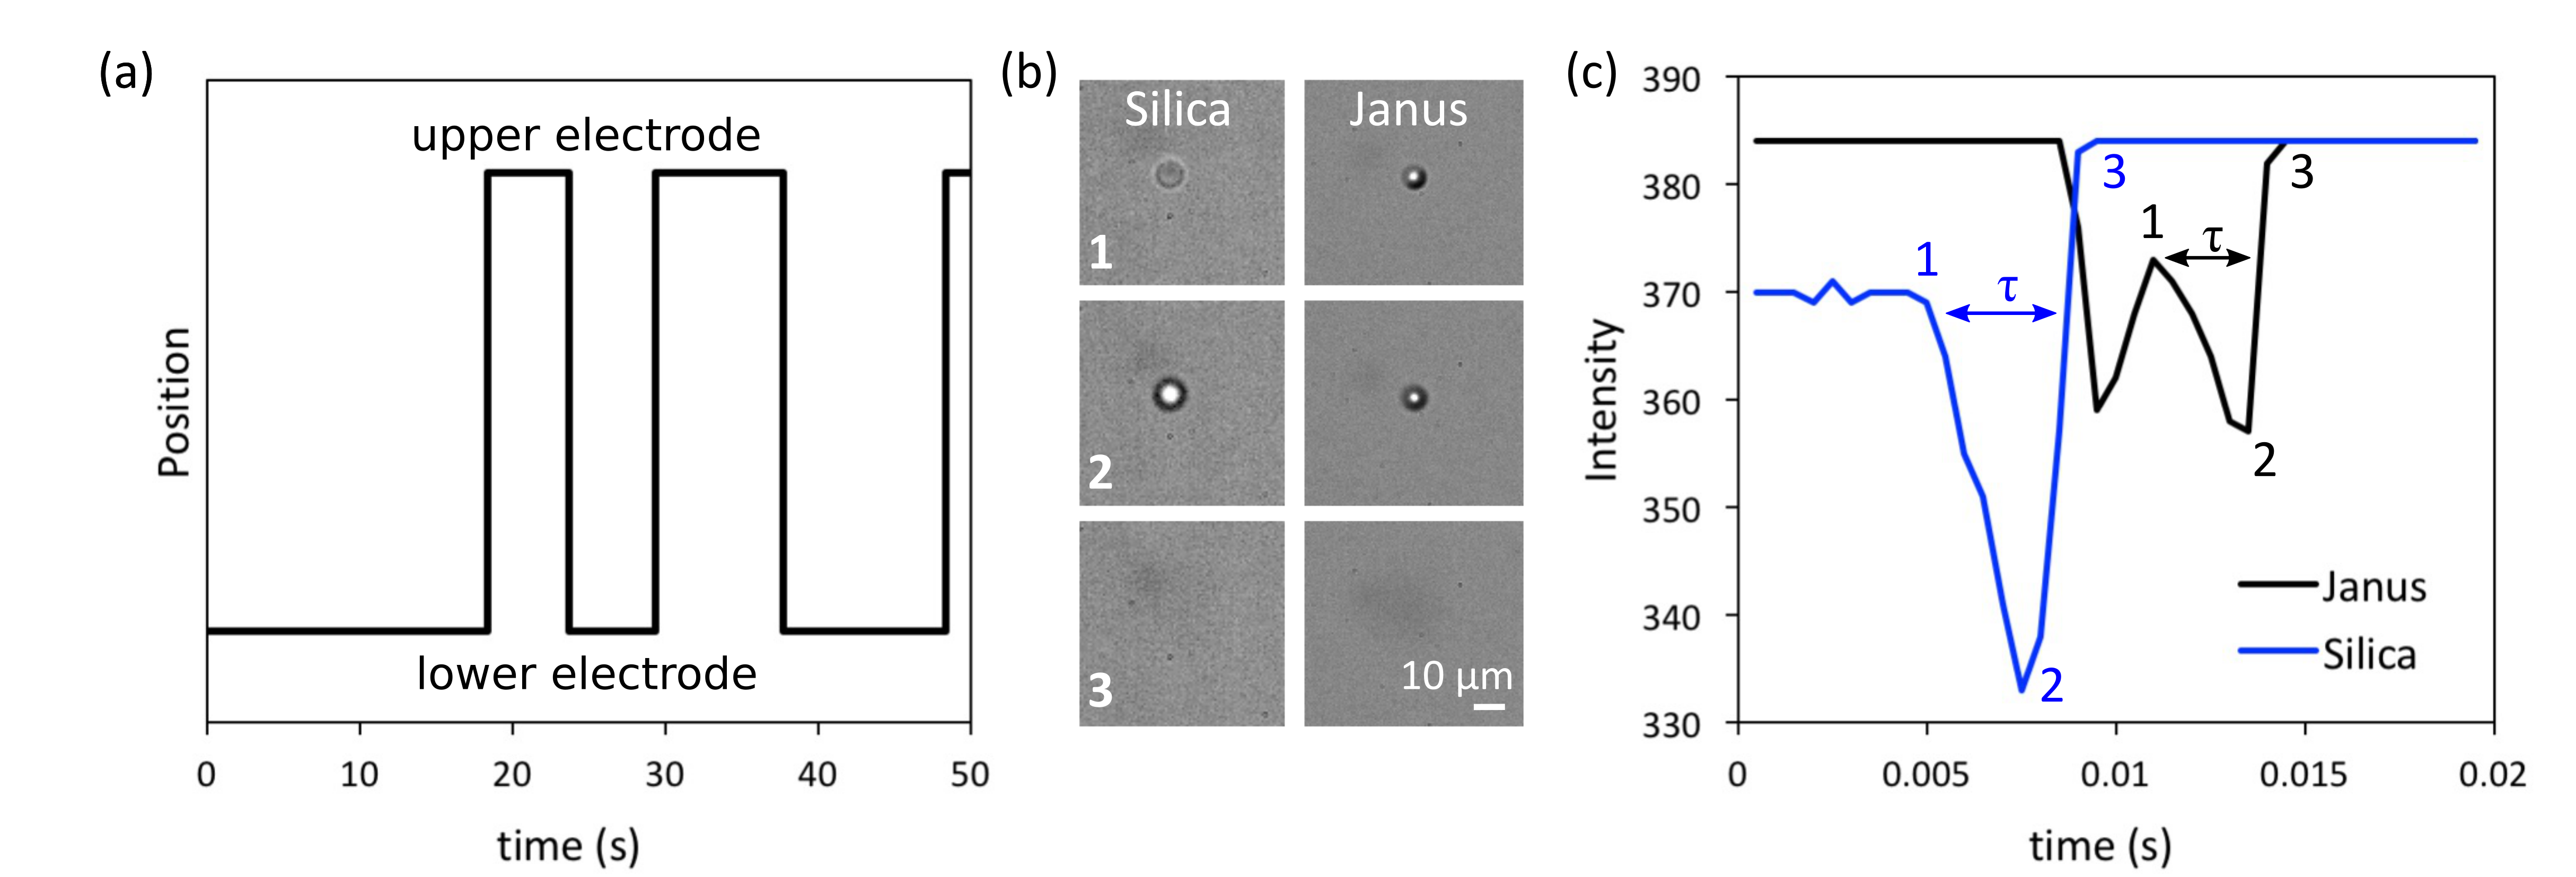
\includegraphics[width=\textwidth]{figures/A1_SilicaParticles.png}
    \caption{(a) A single silica particle oscillates between two parallel electrodes ($V=800~\text{V}$, $H=200~\mu\text{m}$). (b) Microscopy images show a silica particle (left) and a Janus particle (right) near the lower electrode as they move out of focus; the different particles leave the electrode surface at similar rates. (c) The average intensity vs.~time for the image series in (b). The characteristic time $\tau$ required for the particle to move out of focus is indicated for each particle.}
    \label{fig:Silica}
\end{figure}


%%%%%%%%%%%%%%%%%%%%%%%%%%%%%%
%%%%%%%%%%%%%%%%%%%%%%%%%%%%%%
\subsection{\new{Variations in Janus Particle Dynamics}}

In experiment, we measured the lateral displacement $\Delta_i$ and the oscillation period $T_i=t_{i+1}-t_{i}$ for the $i^{\text{th}}$ oscillation of each particle.
These measured quantities show significant variations both from one oscillation to the next and from particle to particle. 
Here, we quantify these variations and discuss their likely origins.
Figure \ref{fig:Variations} shows the displacement and period for several different particles during 50 oscillation cycles.
For each particle, there was little or no correlation between the displacement and the period; the coefficient of determination averaged over 10 different particle was $\langle R^2\rangle=0.29$.
Similarly, the average displacement of each particle was not correlated to its average period ($R^2 = 0.22$).
These results suggests that variations in the displacement are largely independent from those in the period; these quantities can therefore be considered separately.
For each particle, we computed the standard deviation of displacement and the period for the 50 oscillation cycles.
For the displacement, the standard deviation ranged from $0.13~\mu\text{m}$ ($20\%$ of the mean) to $0.81~\mu\text{m}$ ($60\%$) with an average variation of $0.50~\mu\text{m}$ ($40\%$).
For the period, the standard deviation ranged from $2.0~\mu\text{s}$ ($8\%$ of the mean) to $9.7~\mu\text{s}$ ($28\%$) with an average variation of $4.8~\mu\text{s}$ ($15\%$).

\begin{figure}[h]
    \centering
    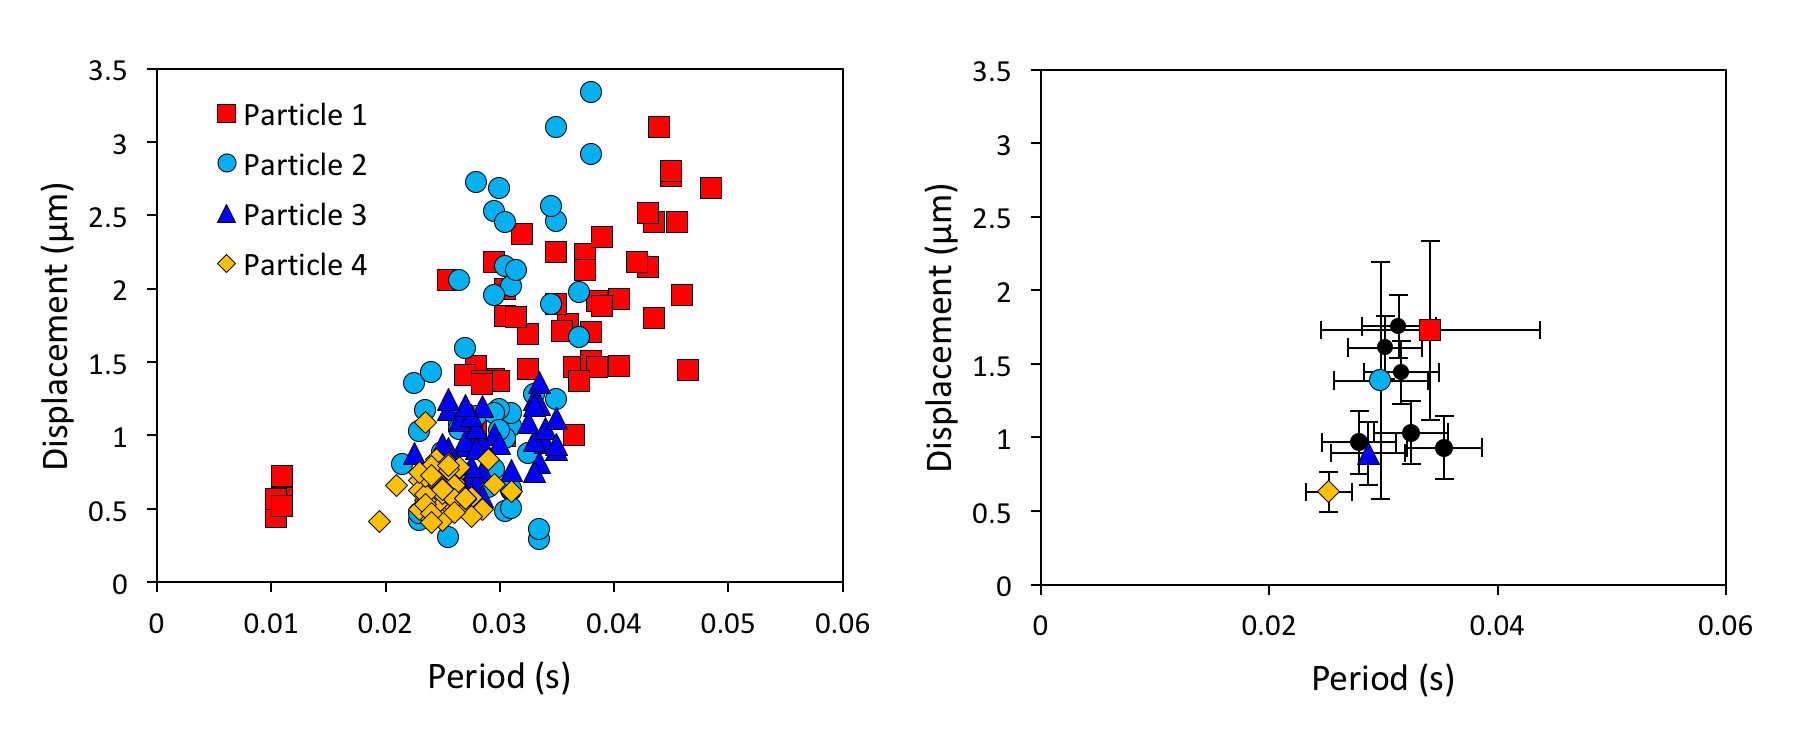
\includegraphics[width=\textwidth]{figures/A1_VariationPlots.png}
    \caption{(left) Lateral displacement $\Delta$ vs.~oscillation period $T$ for four particles showing 50 oscillation cycles. (right) Average displacement vs.~average period for 10 particles; error bars denote one standard devation above/below the mean. Here, the applied voltage is $V=800~\text{V}$ and the electrode separation is $H=200~\mu\text{m}$.}
    \label{fig:Variations}
\end{figure}

Variations in the oscillation period were likely due to differences in the the amount of charge acquired by the particle during electrical contact with the electrode \autocite{drews2015contact}.
The charging process is believed to proceed by an electric discharge, which occurs when the local electric field between the particle surface and the electrode exceeds some critical value.
Importantly, this discharge is extinguished before the particle can acquire its ``full'' equilibrium charge (\emph{i.e.}, that expected when the particle potential is equal to that of the electrode).
Variations in the duration of the discharge may cause variability in the amount of charge acquired by the particle.
The oscillation period is expected to depend inversely on the particle charge as $T\propto q^{-1}$.
By contrast, the lateral displacement is only weakly dependent on the charge (Fig.~\ref{fig:Displacement}).

There are several possible sources of variation in the particles' lateral displacement.
First, the resolution of the microscope images ($0.25~\mu\text{m per pixel}$) limits our ability to identify the location of the particle center with accuracy greater than ${\sim}0.25~\mu\text{m}$.
Second, the displacement depends on the separation $\delta$ between the particle and the electrode at electrical contact; this distance is likely variable owing to the stochastic nature of the electric discharge that mediates charge transfer.
Third, particle to particle variation may arise due to imperfections in the metallic hemisphere and/or charge on the dielectric hemisphere; these effects are thought to be responsible for the circular trajectories observed in experiment.

%%%%%%%%%%%%%%%%%%%%%%%%%%%%%%
%%%%%%%%%%%%%%%%%%%%%%%%%%%%%%
\subsection{\new{Native Charge on the Dielectric Hemisphere}}

In our analysis, we neglected effects due to native charge on the dielectric hemisphere of the Janus particle.
Here, we provide order-of-magnitude estimates to support this assumption.
We assume that the zeta potential $\zeta$ of a homogeneous dielectric sphere is on the order of the thermal potential $k_BT/e\sim25~\text{mV}$. 
Using the linear Poisson-Boltzmann equation \autocite{berg2014effects}, the zeta potential is related to the surface charge as $\sigma=\varepsilon(1+\kappa a)\zeta/a$, where $\kappa$ is the Debye screening length. 
For micron sized particles in mineral oil, the screening length is larger than particle (see estimate below) such that $\sigma\sim \zeta/a$. Alternatively, the charge density acquired by a conductive sphere upon contact with an electrode is $\sigma_c\sim \varepsilon E$. 
The native charge is therefore negligible when $Ea/\zeta \gg 1$; in the present experiments, this ratio is of order $10^3$.
As discussed above (Section \ref{sec:Dielectric}), significant amounts of charge may be present on the dielectric surface due to contact charging with the electrode.

The Debye screening length in mineral oil is estimated to be $\kappa^{-1}\sim 20~\mu\text{m}$ based on the definition $\kappa = (2e^2 n_0/\varepsilon k_B T)^{1/2}$ where $n_0\sim10^{15}~\text{ions/m}^3$ is the ion density. 
The ion density is estimated from the measured electrical conductivity of mineral oil as $K = e n_0 / \lambda\sim 10^{-12}~\text{S/m}$ where $e$ is the elementary charge, and $\lambda\sim6\pi\eta a_i$ is an approximate ion drag coefficient in mineral oil (viscosity, $\eta = 0.027~\text{Pa s}$; ion radius, $a_i = 0.2~\text{nm}$) \autocite{cartier2014microfluidic}.  


%%%%%%%%%%%%%%%%%%%%%%%%%%%%%%
%%%%%%%%%%%%%%%%%%%%%%%%%%%%%%
\subsection{\new{Electrothermal Effects}}

It is unlikely that electrothermal effects contribute significantly to the particle motions observed in experiment.
During contact charging, the flow of charge to/from the particle heats the fluid near the point of contact possibly inducing thermal flows. 
An order-of-magnitude estimate reveals the relevant temperature variations to be quite small.  
Charge of order $q\sim4\pi a^2 E$ is transferred to the particle over a characteristic voltage $aE$. 
The total energy dissipated by Joule heating is estimated as the product of these quantities, $4\pi a^3 E^2$, which is of order $4\times10^{-13}~\text{J}$ (assuming $a = 4~\mu\text{m}$, $E = 5~\text{V/}\mu\text{m}$).  
Equating the energy dissipated by Joule heating to the adiabatic heating of mineral oil in a volume comparable to the particle size yields a temperature increase of $T\sim4\pi a^3E^2/\rho c_p a^3\sim 10^{-3}~\text{K}$ (assuming density $\rho = 850~\text{kg/m}^3$ and specific heat $c_p = 1700~\text{J/kgK}$) for mineral oil).






%%%%%%%%%%%%%%%%%%%%%%%%%%%%%%
%%%%%%%%%%%%%%%%%%%%%%%%%%%%%%

\section{Theoretical Details}

%%%%%%%%%%%%%%%%%%%%%%%%%%%%%%
%%%%%%%%%%%%%%%%%%%%%%%%%%%%%%
\subsection{Electrostatics}

%%%%%%%%%%%%%%%%%%%%%%%%%%%%%%
\subsubsection{Charged Janus Particle in a Uniform Electric Field}
\label{sec:unbounded}

We consider a metallodielectric Janus sphere of radius $a$ positioned in an unbounded dielectric fluid and subject to a uniform electric field $\ve{E}^{\infty}$.
One half of the sphere is a perfect conductor; the other is a dielectric with permittivity $\varepsilon$ assumed equal to that of surrounding fluid. 
The conductive hemisphere has a constant charge $q$, which is acquired on electrical contact with an electrode surface (see below).
Let $\ve{b}$ be the unit vector directed from the center of the particle towards the pole on the conductive hemisphere.
The electric potential $\Phi$ within the dielectric fluid is governed by the Laplace equation
\begin{equation}
    \nabla^2\Phi = 0. \label{eq:laplace}
\end{equation}
Far from the particle, the potential is given by
\begin{equation}
    \Phi(\ve{r}) = \Phi^{\infty}(\ve{r}) = -\ve{r}\cdot\ve{E}^{\infty} \text{ for } r\rightarrow\infty,
\end{equation}
where $r=0$ at the center of the sphere.
The potential on the conductive hemisphere is a constant $\Phi(\ve{r})=\Phi_p$, such that the total charge satisfies 
\begin{equation}
    q = \int_{S_p} -\varepsilon \ve{n}\cdot\nabla\Phi dS,\label{eq:charge}
\end{equation}
where $\ve{n}$ is the unit normal vector directed outward from the surface of the conductive hemisphere $S_p$.

The above equations can be solved for the potential $\Phi$ and the electric field $\ve{E}=-\nabla\Phi$ surrounding the conductive hemisphere of the of the particle.
The net electric force on the Janus particle can then be computed by integrating the Maxwell stress over the conductive hemisphere as
\begin{equation}
    \ve{F} =  \int_{S_p} \frac{1}{2}\varepsilon E^2 \ve{n} dS = q \ve{E}^{\infty}.
\end{equation}
Similarly, the electric torque about the particle center can be computed as
\begin{equation}
    \ve{L} =  \int_{S_p} \frac{1}{2}\varepsilon E^2 (\ve{r}\times \ve{n}) dS = L \frac{\ve{b}\times\ve{E}^{\infty}}{|\ve{b}\times\ve{E}^{\infty}|}.
\end{equation}

Scaling lengths by $a$, the electric potential by $a E^{\infty}$, and charge by $q_s=4\pi\varepsilon a^2 E^{\infty}$, this electrostatic problem is fully characterized by two dimensionless quantities: (i) the orientation of the Janus sphere relative to the field as characterized by the angle $\alpha$ (where $\ve{b}\cdot\ve{E}^{\infty} = E^{\infty} \cos\alpha$), and (ii) the scaled charge on the particle $q / q_s$.
Furthermore, owing to the linearity of the Laplace equation, the torque on the particle is a linear function of the charge and may be expressed as
\begin{equation}
    L(\alpha,q) = \varepsilon a^3 {E^{\infty}}^2 \left[g_0^{\infty}(\alpha) + g_1^{\infty}(\alpha) \left(\frac{q}{q_s}\right) \right], \label{eq:torqueInf}
\end{equation}
where $g_0^{\infty}(\alpha)$ and $g_1^{\infty}(\alpha)$ are dimensionless functions. These functions were computed numerically using a commercial finite element solver (COMSOL) as illustrated in Figure \ref{fig:TorqueFunctions}.

\begin{figure}[h]
    \centering
    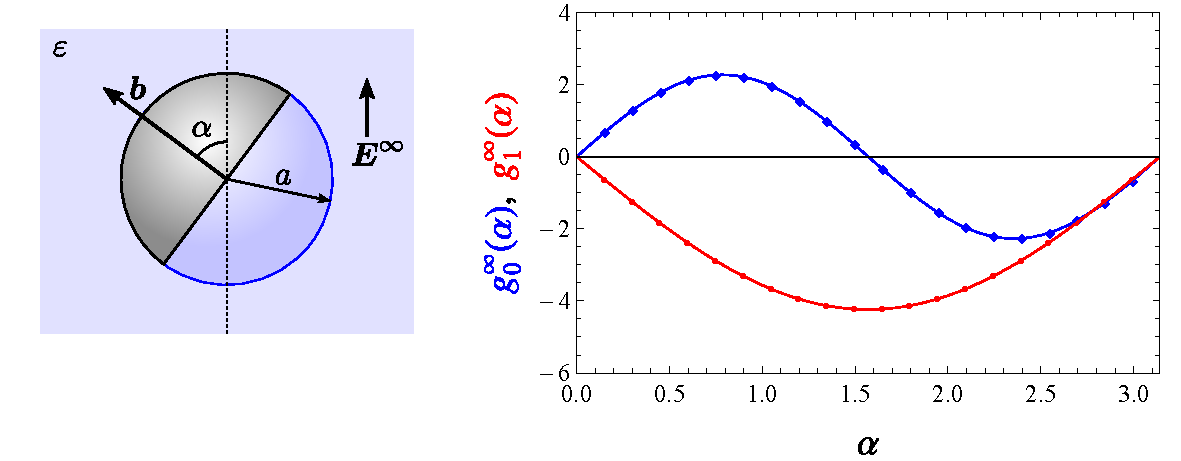
\includegraphics[height=5cm]{figures/A1_Unbounded.pdf}
    \caption{(\emph{left}) Schematic illustration of a Janus particle in a uniform electric field $\ve{E}^{\infty}$.  (\emph{right}) Dimensionless functions $g_0^{\infty}(\alpha)$ and $g_1^{\infty}(\alpha)$ used in equation (\ref{eq:torqueInf}) to compute the electric torque $L$ on a Janus sphere in an unbounded medium. The markers are computed using COMSOL; the solid curves are least squares fits of the form $g_0^{\infty}(\alpha)=A\sin(2\alpha)$ and $g_1^{\infty}(\alpha)=B \sin(\alpha)$ (with $A=2.27$ and $B=-4.24$).}
    \label{fig:TorqueFunctions}
\end{figure}


Depending on the magnitude of the charge $q$, the Janus sphere may adopt different stable orientations, for which $L(\alpha) = 0$ and $L'(\alpha) < 0$.  When the net charge on the particle is zero, the particle orients perpendicular to the applied field ($\alpha = \pi/2$). Conversely, when the particle charge is large such that $q\gg q_s$, the particle prefers to align parallel with the applied field ($\alpha \rightarrow 0$ for $q>0$ or $\alpha \rightarrow \pi$ for $q<0$). For intermediate charges (like those found in the experiment), the stable orientation of the particle lies between these limiting extremes -- namely, $0<\alpha<\pi/2$ for positively charged particles. Importantly, when the sign of the particle is reversed, it experiences an electric torque that rotates the particle into a newly stable orientation. It is this rotational motion in proximity to the electrode surface that results in the translational motion of the particle.


%%%%%%%%%%%%%%%%%%%%%%%%%%%%%%
\subsubsection{Contact-Charging of a Janus Particle at an Electrode Surface}

The charge acquired by a metallodielectric Janus sphere on contact with either of the coplanar electrodes can be estimated by assuming that charge flows onto / from the conductive hemisphere until its potential is equal to that of the proximal electrode.
Specifically, we consider the charging of a particle positioned at height $z_p = a + \delta$ above a planar electrode at $z=0$; here, $\delta$ is the surface separation, which is assumed small compared to the particle radius ($\delta\ll a$).
The potential on the electrode and the conductive hemisphere are assumed to be zero
\begin{equation}
    \Phi(\ve{r}) = 0 \text{ for } \ve{r} \in \text{electrode or particle}. \label{eq:nearBC}
\end{equation}
Far from the electrode, the potential approaches that due to the applied field $\ve{E}^{\infty}=E^{\infty}\ve{e}_z$
\begin{equation}
    \Phi(\ve{r}) = -z E^{\infty} \text{ for } \ve{z} \rightarrow \infty. \label{eq:farBC}
\end{equation}
Solving the Laplace equation (\ref{eq:laplace}) subject to boundary conditions (\ref{eq:nearBC}) and (\ref{eq:farBC}), the charge $q$ on the particle is then computed using equation (\ref{eq:charge}).
For a fixed surface separation $\delta$, the charge acquired on contact depends only on the orientation of the particle relative to the surface as illustrated in Figure \ref{fig:ContactCharge}.

\begin{figure}[h]
    \centering
    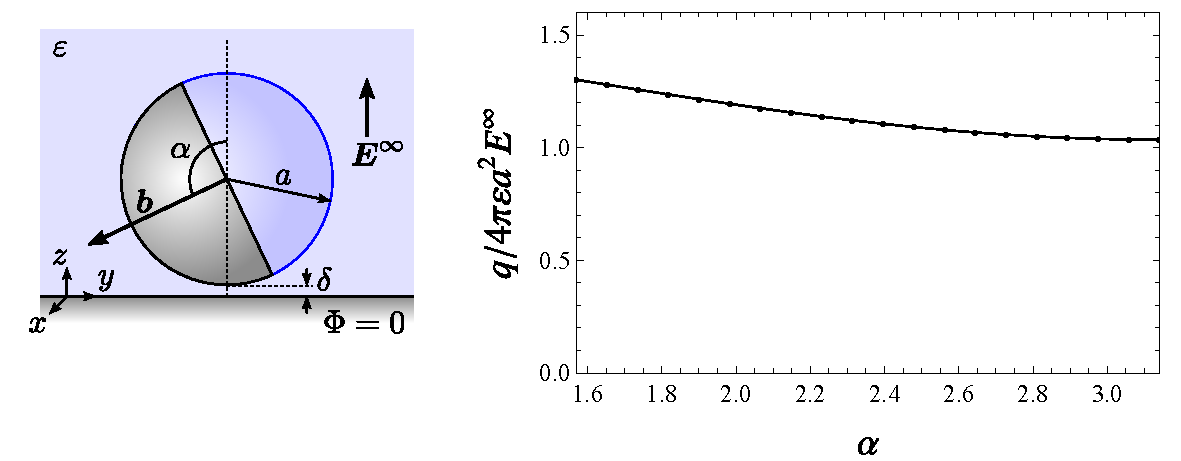
\includegraphics[height=5.5cm]{figures/A1_ContactCharge.pdf}
    \caption{(\emph{left}) Schematic illustration of a Janus particle in electrical contact with a planar electrode. (\emph{right}) Charge acquired by the particle (scaled by $4\pi \varepsilon a^2 E^{\infty}$) as a function of its orientation.  Here, the surface separation is $\delta= 0.02 a$ (similar results are obtained for other $\delta$ provide $\delta\ll a$). The plot markers are computed using COMSOL; the solid curve is a least squares fit of the form $y=A + B \cos x$ (with $A=1.30$ and $B=0.266$).}
    \label{fig:ContactCharge}
\end{figure}


%%%%%%%%%%%%%%%%%%%%%%%%%%%%%%
\subsubsection{Electric Force and Torque on a Janus Particle at Finite Surface Separations}

In section \ref{sec:unbounded}, we evaluated the force and torque on a Janus particle in an unbounded medium subject to a uniform electric field.  We now consider the case when the surface of the particle is separated by a dimensionless distance $\xi=(z_p-a) / a$ from a grounded plane.  The force and torque on the particle depends on the particle orientation $\alpha$, on the surface separation $\xi$, and the particle charge $q$ as
\begin{gather}
    F(\alpha,h,q) = \varepsilon a^2 {E^{\infty}}^2 \left[f_0(\alpha,\xi) + f_1(\alpha,\xi) \left(\frac{q}{q_s}\right)  + f_2(\alpha,\xi)\left(\frac{q}{q_s}\right)^2 \right], \label{eq:Force}
    \\
    L(\alpha,h,q) = \varepsilon a^3 {E^{\infty}}^2 \left[g_0(\alpha,\xi) + g_1(\alpha,\xi) \left(\frac{q}{q_s}\right)  + g_2(\alpha,\xi)\left(\frac{q}{q_s}\right)^2 \right].\label{eq:Torque}
\end{gather}
Here, the dimensionless functions $f_i(\alpha,\xi)$ and $g_i(\alpha,\xi)$ were computed numerically and approximated by parametric interpolants of the form
\begin{gather}
    f_i(\alpha,\xi) = \sum_{j=0}^{15}\sum_{k=0}^5 A_{ijk} \frac{\cos j\alpha}{\xi^k},\label{eq:ForceInterpolant}
    \\
    g_i(\alpha,\xi) = \sum_{j=1}^{15}\sum_{k=0}^5 B_{ijk} \frac{\sin j\alpha}{\xi^k},\label{eq:TorqueInterpolant}
\end{gather}
where the coefficients $A_{ijk}$ and $B_{ijk}$ are determined by linear least squares regression (Figure \ref{fig:ForceTorque}). In the limit of large surface separations ($h\rightarrow\infty$), the solution approaches the result described in the previous section 
\begin{gather}
    f_0(\alpha,h)\rightarrow0,~~ f_1(\alpha,h)\rightarrow4\pi,~~ f_2(\alpha,h)\rightarrow0,
    \\
    g_0(\alpha,h)\rightarrow g_0^{\infty}(\alpha),~~ g_1(\alpha,h)\rightarrow g_1^{\infty}(\alpha),~~ g_2(\alpha,h)\rightarrow0.
\end{gather}
Knowledge of the force and torque is necessary to describe the translational and rotational dynamics of a Janus particle as it approaches an electrode, reverses charge, and returns towards the opposite electrode.

\begin{figure}
    \centering
    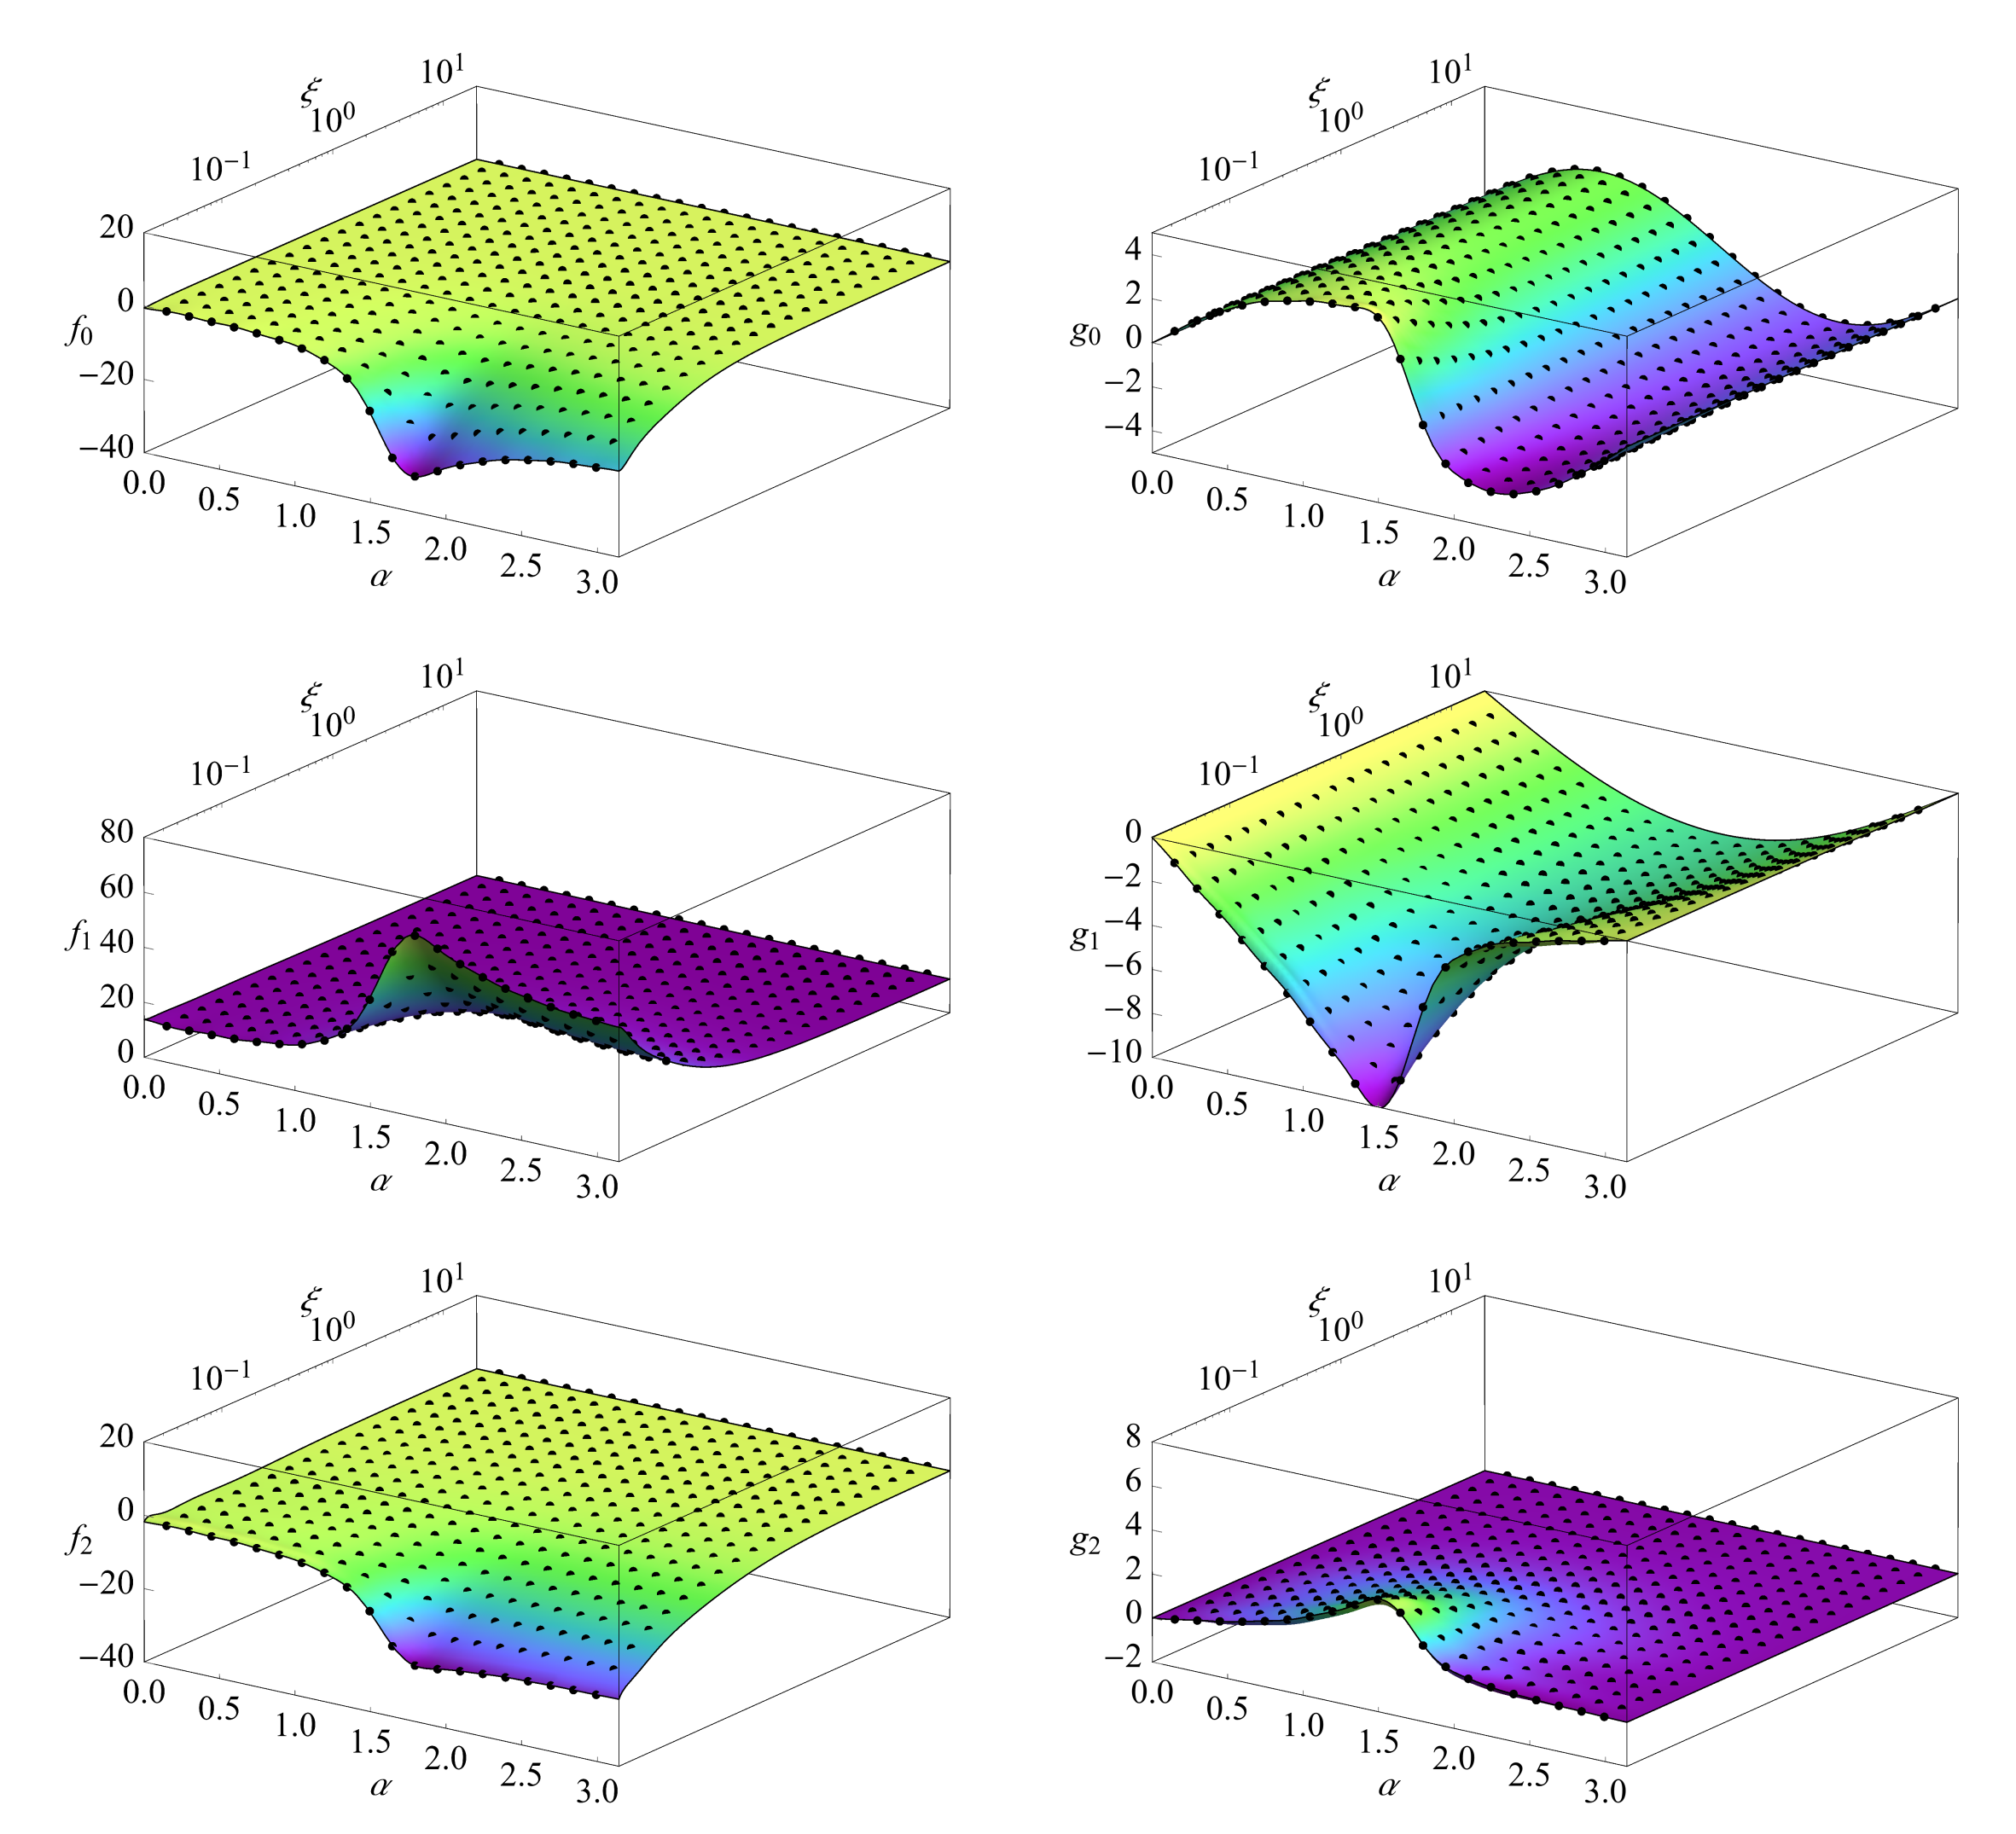
\includegraphics[width=15cm]{figures/A1_ForceTorque.png}
    \caption{Dimensionless functions $f_i(\alpha,\xi)$ and $g_i(\alpha,\xi)$ used in equations (\ref{eq:Force}) and (\ref{eq:Torque}) to evaluate the force and torque on a charged Janus particle near a grounded plane. The parameter $\alpha$ describes the orientation of the particle; $\xi=(zp-a)/a$ describes its separation from the surface. The markers are computed numerically using COMSOL; the surfaces are least squares interpolants given by equations (\ref{eq:ForceInterpolant}) and (\ref{eq:TorqueInterpolant}).}
    \label{fig:ForceTorque}
\end{figure}


%%%%%%%%%%%%%%%%%%%%%%%%%%%%%%
%%%%%%%%%%%%%%%%%%%%%%%%%%%%%%
\subsection{Hydrodynamics}

At low Reynolds numbers, the electric force $\ve{F}$ and torque $\ve{L}$ acting on the particle gives rise to its translational and rotation motion as described by the linear relation
\begin{equation}
    \begin{bmatrix}
    \ve{F} \\ \ve{L}
    \end{bmatrix}
    =
    \begin{bmatrix}
    \ve{A} & \tilde{\ve{B}}
    \\ 
    \ve{B} & \ve{C}
    \end{bmatrix}
    \cdot
    \begin{bmatrix}
    \ve{U} \\ \ve{\Omega}
    \end{bmatrix}, \label{eq:resistance}
\end{equation}
where $\ve{U}$ and $\ve{\Omega}$ are the translation and rotational velocities of the particle, and  $\ve{A}$, $\ve{B}$, $\tilde{\ve{B}}$, and $\ve{C}$ are hydrodynamic resistance tensors.  For a spherical particle moving near a solid plane ($z=0$), the components of the resistance tensors take the form 
\begin{gather}
    A_{ij} = 6\pi\eta a \left[ X^A \delta_{i3}\delta_{j3} + Y^A (\delta_{ij} - \delta_{i3}\delta_{j3}) \right], 
    \\
    B_{ij} = \tilde{B}_{ji} = 6\pi\eta a^2 \left[ Y^B \varepsilon_{3ij} \right],
    \\
    C_{ij} = 6\pi\eta a^3 \left[  X^C \delta_{i3}\delta_{j3} + Y^C (\delta_{ij} - \delta_{i3}\delta_{j3}) \right], 
\end{gather}
where $\delta_{ij}$ is the Kronecker delta, and $\varepsilon_{ijk}$ is the permutation symbol. The coefficients $Y^A$ and $Y^B$ describe, respectively, the dimensionless force and torque on a sphere translating \emph{parallel} to a solid plane surface \autocite{ONeill1964a}. The coefficient $Y^C$ describes the torque on a sphere rotating about an axis \emph{parallel} to the surface \autocite{Dean1963}. The coefficient $X^A$ describes the force on a sphere translating \emph{perpendicular} to the surface \autocite{Brenner1961a}.  Finally, $X^C$ describes the torque on a sphere rotating about an axis \emph{perpendicular} to a the surface \autocite{Jeffrey1915}. These coefficients depend only on the dimensionless surface separation $\xi = (z_p - a)/a$ as illustrated in Figure \ref{fig:resistance}. 

\begin{figure}[h]
    \centering
    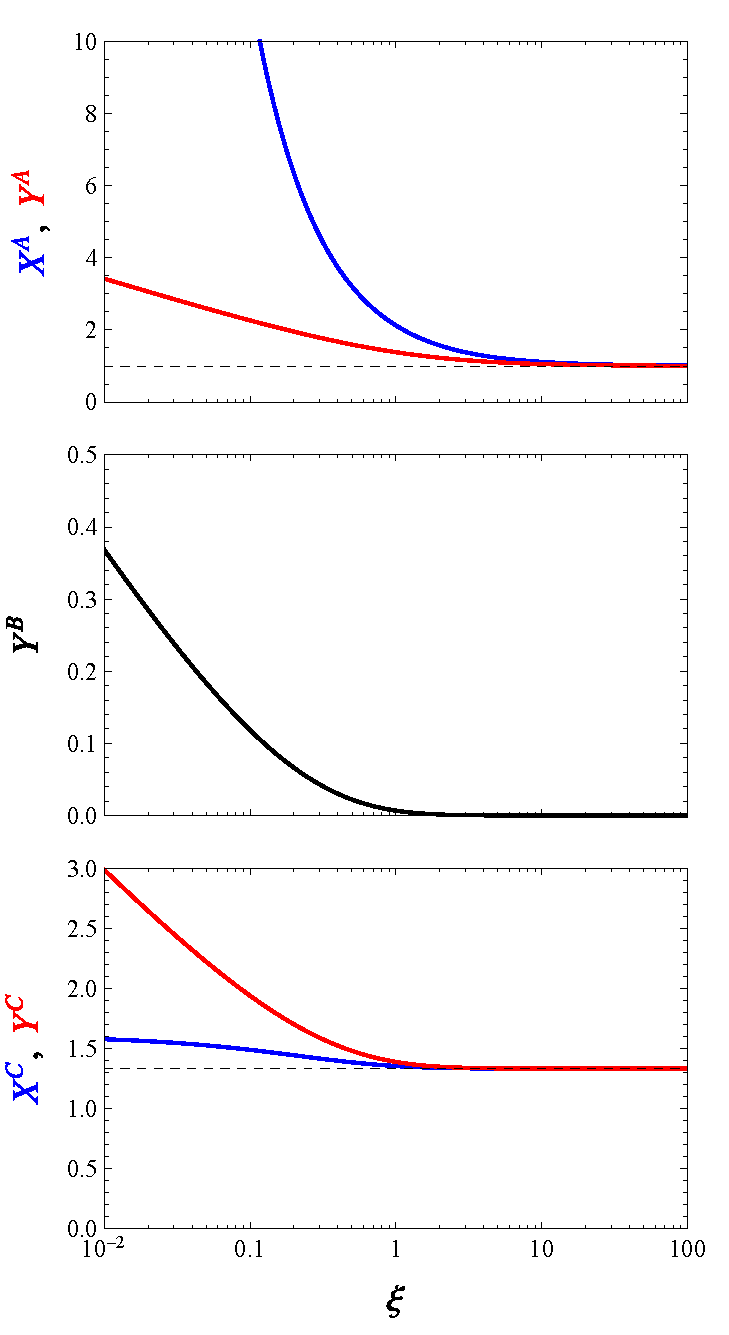
\includegraphics[width=7cm]{figures/A1_resistance.pdf}
    \caption{Resistance coefficients for a sphere of radius $a$ as a function of the surface separation $\xi=(z_p-a)/a$ with plane surface at $z=0$. The dashed lines denote the behavior of an isolated particle in an unbounded medium.}
    \label{fig:resistance}
\end{figure}

%%%%%%%%%%%%%%%%%%%%%%%%%%%%%%
%%%%%%%%%%%%%%%%%%%%%%%%%%%%%%
\subsection{Particle Dynamics}

We now consider the dynamics of a single Janus particle as it approaches the plane electrode at $z=0$, makes electrical contact, and then moves off towards the opposite electrode. We assume that the particle director $\ve{b}$ lies in the $yz$ plane throughout the ``collision'' (Figure \ref{fig:Collision}).  For this geometry, symmetry implies that $F_x=F_y=L_y=L_z=0$, and equation (\ref{eq:resistance}) can be inverted to obtain
\begin{align}
    U_y &= \dot{y}_p =- \frac{1}{6\pi\eta a^2} \left(\frac{Y^B L_x}{Y^A Y^C - {Y^B}^2}\right),
    \\
    U_z &= \dot{z}_p = \frac{1}{6\pi\eta a} \left( \frac{F_z}{X^A}\right),
    \\
    \Omega_x &= \dot{\alpha} = \frac{1}{6\pi\eta a^3} \left(\frac{Y^A L_x}{Y^A Y^C - {Y^B}^2} \right).
\end{align}
Here, resistance coefficients depend on the dimensionless separation $\xi$ between the particle and the surface; the force and torque depend on both the surface separation $\xi$ and the angle $\alpha$. These dynamical equations can be integrated numerically to describe the translational and rotational motion of the particle in time. 

Figure \ref{fig:Collision} illustrates the dynamics of two such particle ``collision'' with the electrode surface. Initially, the particle is negatively charged.  It moves towards the surface with a fixed orientation until reaching a finite surface separation $\delta$, at which point its charge reverses sign. Upon the change in polarity, the particle  rotates towards its new stable orientation.  The rotation of the particle in close proximity to the plane surface results in a net displacement $\Delta$ away from the conductive hemisphere of the particle.  Note that the magnitude of this displacement depends on the particle charge $q$ and the surface separation $\delta$ at contact (Figure \ref{fig:Displacement}).

\begin{figure}[h]
    \centering
    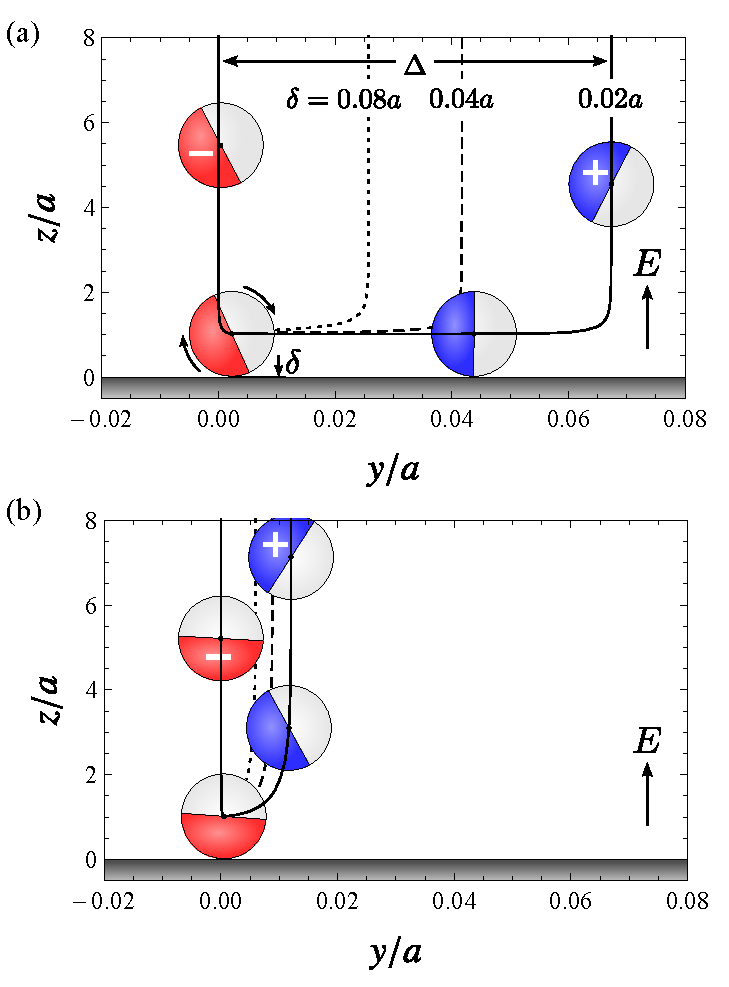
\includegraphics[width=9cm]{figures/A1_Collision.pdf}
    \caption{ Simulated particle ``collisions'' with the lower electrode for a particle charge (a) $q=\pm0.5q_s$ and (b) $q=\pm1.058q_s$. The solid curve shows the trajectory of the particle center; the orientation of the particle at different points along the trajectory is illustrated graphically. The net particle displacement $\Delta$ depends on the surface separation $\delta$ at ``contact'' when the particle charge reverses polarity. Note that for clarity the $z$ and $y$ axes use different scales.}
    \label{fig:Collision}
\end{figure}

\begin{figure}[h]
    \centering
    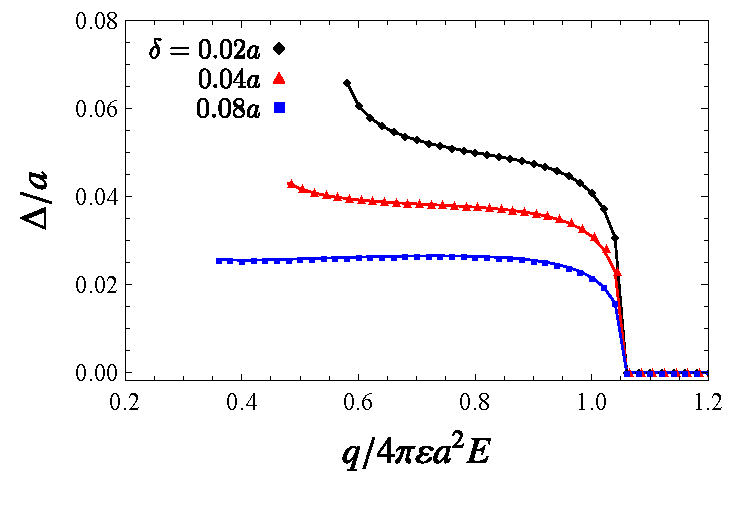
\includegraphics[width=9cm]{figures/A1_Displacement.pdf}
    \caption{Net displacement $\Delta$ of a Janus particle during a single particle ``collision`` as a function of the particle charge $q$ for three different contact separations $\delta$. Note that when the charge acquired is below some critical value (open circles), the particle remains bound to the electrode \autocite{drews2015contact}.}
    \label{fig:Displacement}
\end{figure}




%%%%%%%%%%%%%%%%%%%%%%%%%%%%%%
%%%%%%%%%%%%%%%%%%%%%%%%%%%%%%




\end{appendices}